% \input{\pSections "sec-radiation"}

\section{Radiation}

\begin{frame}{Energy Out, Energy In}
    \centering
    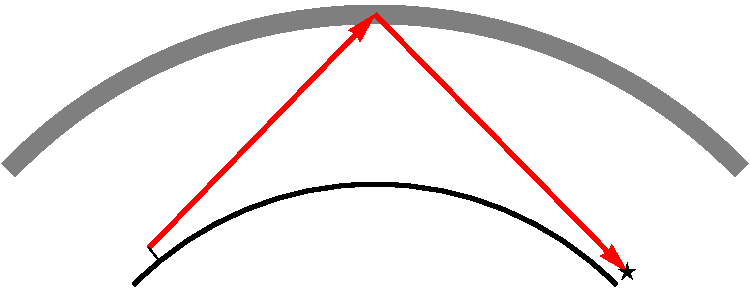
\includegraphics[ width = 0.7\textwidth ]{ \pLocalGraphics/energy-out.pdf } \\[1em]
    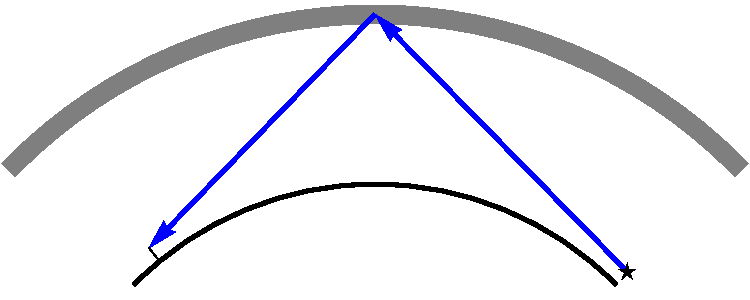
\includegraphics[ width = 0.7\textwidth ]{ \pLocalGraphics/energy-in.pdf } \\[1em]
   % \textit{\small Radar transmits energy outward (blue), receives scattered energy inward (red).}
\end{frame}

\begin{frame}{Energy Out, Energy In}
    	\begin{enumerate}
		\item radar (left) {\color{red}{irradiates}} target (star)
		\item {\color{blue}{backscatter}} travels from target to radar
	\end{enumerate}

\end{frame}


%     %     %     %     %     %     %     %     %
\subsection{Effective Radar Cross Section}

\begin{frame}\frametitle{Radar Cross Section: Definition}
	\begin{equation}
		\sigma_{\star} = 4\pi\lim\limits_{r\to\infty} r^{2} \left|\frac{\textcolor{red}{E_{\text{incident}}}}{\textcolor{blue}{E_{\text{scattered}}}}\right|^{2}
	\end{equation}
	\\[20pt]
	\cite[(2.36)]{skolnik1962introduction}	
\end{frame}
		%
\begin{frame}\frametitle{Radar Cross Section: Discussion}
	\begin{itemize}
		\item Radar cross section is a {\bl{far field}} phenomenon
		\item Assumes {\bl{single polarization}} to and from target
		\item Target is {\bl{completely metallic}}: \\$E$ field results from surface currents
		\item Shape is {\bl{quasi-dimensional}}
			\begin{itemize}
				\item Dimensions in two known directions
				\item Dish antennae, solar panels, booms
			\end{itemize}
		\item {\bl{Resonant scattering}}: \\Ratio of typical dimension to wavelength $\approx$ 1 
		\item \cite[\S 4.6]{kolosov1987}
	\end{itemize}	
\end{frame}

\begin{frame}{Radar Cross Section: Conceptual Overview}
    \small
    \begin{itemize}
        \item \textcolor{blue}{Radar Basics:}
            \begin{itemize}
                \item Transmit energy \cite[p. 21]{skolnik1962introduction}.
                \item Receive scattered signal.
                \item Direction, strength → object properties \cite[p. 45]{knott2004radar}.
            \end{itemize}
        \item \textcolor{blue}{What is RCS?}
            \begin{itemize}
                \item Measures object "visibility" to radar \cite[Section 2]{cite-trcs}.
                \item Depends on:  
                    \begin{itemize}
                        \item Material  
                        \item Geometry  
                        \item Orientation \cite[pp. 3-4]{peebles2007radar}.
                    \end{itemize}
            \end{itemize}
        \item \textcolor{blue}{Key Question:}
            Power reflected vs. power transmitted.
    \end{itemize}
\end{frame}

\begin{frame}{Factors Influencing Radar Cross Section}
    \small
    \begin{itemize}
        \item \textcolor{blue}{Shape:}
            \begin{itemize}
                \item Smooth → directional reflection \cite[p. 47]{knott2004radar}.
                \item Complex → scattered energy.
            \end{itemize}
        \item \textcolor{blue}{Material:}
            \begin{itemize}
                \item Metal → strong reflection.
                \item Absorbers → reduced RCS \cite[Section 3.2]{knott2004radar}.
            \end{itemize}
        \item \textcolor{blue}{Size vs. Wavelength:}
            \begin{itemize}
                \item Large → high scattering.
                \item Small → "invisible" (Rayleigh scattering) \cite[p. 188]{kolosov1987}.
            \end{itemize}
        \item \textcolor{blue}{Orientation:}
            \begin{itemize}
                \item Aligned → max RCS \cite[Eq. 2.1]{knott2004radar}.
                \item Tilted → min RCS \cite[p. 22]{skolnik1962introduction}.
            \end{itemize}
        \item \textcolor{blue}{Radar Parameters:}
            \begin{itemize}
                \item Frequency, polarization, incidence angle \cite[p. 45]{cite-trcs}.
            \end{itemize}
    \end{itemize}
\end{frame}


%     %     %     %     %     %     %     %     %
\subsection{Linear Independence}
	
%     %     %     %     %     %     %     %     %
\subsection{Configuring Mercury MoM}

\begin{frame}
	\frametitle{Input files}
	\begin{enumerate}
			%
		\item \texttt{B-20.geo}
		\begin{enumerate}
			\item Points to facet file
			\item Configure linear algebra solver
			\item Radar frequency range
			\item Angular sampling ranges
			\item Boundary conditions
			\item Mono-- or Bistatic
			\item Surface or Volume integral elements
			\item Length units
		\end{enumerate}
			%
		\item \texttt{B-20.facet}
		\begin{enumerate}
			\item Vertex list
			\item Face list 
		\end{enumerate}
			%
		\item \texttt{Materials.lib}
		\begin{enumerate}
			\item Permiability
			\item Permittivity
		\end{enumerate}
			%
	\end{enumerate}
\end{frame}

\myFrame{Linear algebra (don't alter)}{\footnotesize{
\begin{table}[htp]
	\begin{center}
		\begin{tabular}{ll}
			\scry{\&MM\_MOM} \\
			\scrg{  bUseACA = .TRUE.,} & \scrg{  nFillThreads = -1,} \\
			\scrg{  bSolve\_ACA = .TRUE.,} & \scrg{  nFillMKLThreads = 1,} \\
			\scrg{  bOutOfCore = .TRUE.,} & \scrg{  nLUThreads = -1,} \\
			\scrg{  bNormalizeToWaveLength = .FALSE.,} & \scrg{  nLUMKLThreads = 1,} \\
			\scrg{  bNormalize             = .FALSE.,} & \scrg{  nRHSThreads = 1,} \\
			\scrg{  dCloseLambda  = 0.100000,} & \scrg{  nRHSMKLThreads = 1,} \\
			\scrg{  ACA\_Factor\_Tol = 0.000010,} & \scrg{  bOutputACAGrouping     = .FALSE.,} \\
			\scrg{  ACA\_RHS\_Tol = 0.000100,} & \scrg{  bOutputRankFraction    = .FALSE.,} \\
			\scrg{  Point\_Tolerance = 0.001000,} & \scrg{  bLimitLUColumns        = .FALSE.,} \\
			\scrg{  nLargestBlockSize = -1,} & \scrg{  Lop\_Admissibility = WEAK,} \\
			\scrg{  MemorySize\_GB = -1.000000,} & \scrg{  Kop\_Admissibility = CLOSE} \\
			\scrg{  stackSize\_GB = -1.000000,} &  \\
		\end{tabular}
	\end{center}
\end{table}
}}

\myFrame{Memory management (don't alter)}{\footnotesize{
	\scry{\&Scratch\_Memory} \\
	\scrg{  Scratch\_RankFraction\_Z     = 0.300000,} \\
	\scrg{  Scratch\_RankFraction\_LU    = 0.600000,} \\
	\scrg{  Scratch\_RankFraction\_RHS   = 2.000000,} \\
	\scrg{  Scratch\_RankFraction\_Solve = 1.000000,} \\
	\scrg{  MemoryFraction\_Z           = 0.950000,} \\
	\scrg{  MemoryFraction\_Scratch\_LU  = 0.500000,} \\
	\scrg{  MemoryFraction\_LU          = 1.000000,} \\
	\scrg{  MemoryFraction\_RHS         = 0.500000,} \\
	\scrg{  MemoryFraction\_Solve       = 0.900000,}  \\
}}

\myFrame{Quadrature (don't alter)}{\footnotesize{
	\scry{\&QUADRATURE} \\
	\scrg{  NTRISELF    = 7,} \\
	\scrg{ NTRINEAR    = 3,} \\
	\scrg{  NTRIFAR     = 3,} \\
	\scrg{  NTETSELF    = 11,} \\
	\scrg{  NTETNEAR    = 4,} \\
	\scrg{  NTETFAR     = 4,} \\
	\scrg{  NQGAUSS  = 4}  \\
}}

\myFrame{Radar frequencies}{\footnotesize{
	\scry{FREQUENCY} \\
	\scrg{   ghz } \\
	\scrg{   0.003000  0.030000  28   }\scrz{!Freq Start, Freq Stop, Num Frequencies}
}}

\myFrame{Sampling}{\footnotesize{
	\scry{Angle Cut} \\
	\scrg{   1} \\
	\scrg{   0.000000  359.000000  360} \\
	\scrg{   AZIMUTH} \\
	\scrg{   90.000000} \\
}}

\myFrame{Monostatic or bistatic}{\footnotesize{
	\scry{Excitation} \\
	\scrg{   MONOSTATIC}
}}

\myFrame{Boundary Conditions}{\footnotesize{
	\scry{Boundary Conditions} \\
	\scrg{B-20-Materials.lib} \\
	\scrg{4} \\
	\scrg{V\_FREE\_SPACE => Free\_Space} \\
	\scrg{V\_PEC => PEC} \\
	\scrg{V\_PMC => PMC} \\
	\scrg{V\_NULL => NULL} \\
	\scrg{1} \\
	\scrg{0 BC\_PEC V\_FREE\_SPACE}
}}

\myFrame{Final settings}{\footnotesize{
	\begin{table}[htp]
		\begin{center}
			\begin{tabular}{lcl}
				\scry{SIE} & \qquad & \gr{surface integral elements} \\
				\scry{B-20A.facet} && \gr{CAD description} \\
				\scry{m} && \gr{meters} \\
			\end{tabular}
		\end{center}
\end{table}%
}}
	
%     %     %     %     %     %     %     %     %
\subsection{Running Mercury MoM}

\begin{frame}
	\frametitle{Mercury MoM is Single Precision}
	Example: $8$ MHz\\
	Despite exact binary representation \\
	$$ 8_{10} = 1000_{2}$$ \\[10pt]
	\texttt{ Start Frequency =  7.9999994E-03GHz}
\end{frame}

\myFrame{Run sequence - launch}{\tiny{
\scry{\$./MMoM\_4.1.12 b20.geo} \\	
\scrg{--------------------------------------------------------------------------------} \\
\scrg{HOSTNAME                 = 3dd5a4b0d3c8} \\
\scrg{HOSTTYPE                 =} \\
\scrg{CPU                      =} \\
\scrg{OSTYPE                   =} \\
\scrg{MACHTYPE                 =} \\
\scrg{NUMBER\_OF\_PROCESSORS     =} \\
\scrg{OMP\_NUM\_THREADS          =} \\
\scrg{PROCESSOR\_ARCHITECTURE   =} \\
\scrg{PROCESSOR\_IDENTIFIER     =} \\
\scrg{------------ Reporting output in MB from Linux command: vmstat -s -S M ------------} \\
\scrw{        53113 M free memory} \\
}}

\myFrame{Run sequence - sample output}{\tiny{
\scry{  Freq  \phantom{m} =    30.00E+00 MHz} \\
\scrg{  Lambda =     9.99E+00 m  } \\
\scrg{  k   \phantom{mmmm}   =   628.75E-03 m-1} \\
\scrg{subroutine Solve\_SetUp(  Surface, bk, pSys, pD, Nodes )  : ...Finished} \\
\scrg{--------------------------------------------------------------------------------} \\
\scrg{---| Time : Time total for RHS solve} \\
\scrg{---| Twall = 0.0004168 ; Tcpu = 0.0002319 ; Ratio =   1.80} \\
\scrg{--------------------------------------------------------------------------------} \\
\scrg{---| Out Of Core Times:  Diagonal Blocks} \\
\scrg{---|} \\
\scrg{---| nWrites.........................:          2.} \\
\scrg{---| GigaBytes Write.................:          0.} \\
\scrg{---| Write Time (Hr).................:        0.00} \\
\scrg{---| Average Write Rate (MBytes/sec).:         19.} \\
\scrg{---| nReads..........................:          5.} \\
\scrg{---| GigaBytes Read..................:          0.} \\
\scrg{---| Read Time (Hr)..................:      0.0002} \\
\scrg{---| Average Read Rate (MBytes/sec)..:         48.} \\
\scrg{---|} \\
\scrg{--------------------------------------------------------------------------------} \\
\scrg{Z Column Summary IO   0.000E+00   0.000E+00   0.000E+00   0.000E+00   0.000E+00} \\
}}

\myFrame{Run sequence - completion}{\tiny{
\scry{\$./MMoM\_4.1.12 b20.geo} \\
\scrg{--------------------------------------------------------------------------------} \\
\scrg{HOSTNAME                 = 3dd5a4b0d3c8} \\
\scrg{HOSTTYPE                 =} \\
\scrg{CPU                      =} \\
\scrg{OSTYPE                   =} \\
\scrg{MACHTYPE                 =} \\
\scrg{NUMBER\_OF\_PROCESSORS     =} \\
\scrg{OMP\_NUM\_THREADS          =} \\
\scrg{PROCESSOR\_ARCHITECTURE   =} \\
\scrg{PROCESSOR\_IDENTIFIER     =} \\
\scrg{------------ Reporting output in MB from Linux command: vmstat -s -S M ------------} \\
\scrc{        53113 M free memory} \\
}}

\endinput  %  ==  ==  ==  ==  ==  ==  ==  ==  ==
